\documentclass[12pt]{article} % 

\usepackage[hyperfootnotes=false]{hyperref}
\usepackage[margin=1in]{geometry}                                              
\usepackage{amsmath,amsthm,amssymb} 
\usepackage{titlesec}                                                   
\usepackage{bm}
\usepackage{cprotect}
%\usepackage{savetrees}
\usepackage{ bbold }
\usepackage{abstract}
                                           
\usepackage{graphicx}                                                          
\graphicspath{{../data/}}

\usepackage{biblatex}
\bibliography{bib.bib}

\usepackage{tikz}
\usetikzlibrary{arrows,shapes,trees,backgrounds} 
\definecolor{mygray}{gray}{0.6}

\usepackage{listings}
\lstset{basicstyle=\ttfamily,breaklines=true}

%%%%%%%%%%%%%%%%%%%%%%%%%%%%%%%%%%%%%%%%%%%%%%%%%%%%%%%
% Taken from Kitaev Unpaired fermions...
\newenvironment{subfig}[1]%
{\def\subfigLabel{#1}\begin{tabular}[b]{@{}c@{}}}%
	{\\[10pt]\subfigLabel\end{tabular}}

\newsavebox{\TempBox}
\newlength{\TempLength}
%%%%%%%%%%%%%%%%%%%%%%%%%%%%%%%%%%%%%%%%%%%%%%%%%%%%%%%

       

\titleformat{\subsection}[runin]
{\normalfont\large\bfseries}{\thesubsection}{1em}{}

\renewcommand{\bf}{\mathbf}
\renewcommand{\cal}{\mathcal}
\newcommand{\pd}[2]{\frac{\partial #1}{\partial #2}}
\newcommand{\pdn}[3]{\frac{\partial^{#3} #1}{\partial #2^{#3}}}
\newcommand{\pdop}[1]{\frac{\partial}{\partial #1}}
\newcommand{\nd}[2]{\frac{d #1}{d #2}}
\newcommand{\ndn}[3]{\frac{d^{#3} #1}{d #2^{#3}}}
\newcommand{\ndop}[1]{\frac{d}{d #1}}
\newcommand{\dt}{\frac{d}{dt}}
\newcommand{\grad}{\bm\nabla}
\newcommand{\cross}{\times}
\newcommand{\curl}{\grad\cross}
\newcommand{\imp}{\Longrightarrow\quad}
\newcommand{\abs}[1]{\left|#1\right|}
\newcommand{\half}{\frac{1}{2}}
\newcommand{\third}{\frac{1}{3}}
\renewcommand{\th}[1]{\frac{1}{#1}}
\renewcommand{\k}{4\pi\epsilon_0}
\newcommand{\eps}{\epsilon_0}
\newcommand{\intt}{\int_{t_1}^{t_2}}
\newcommand{\inti}{\int_{-\infty}^{+\infty}}
\newcommand{\ex}[1]{\left\langle #1 \right\rangle}
\renewcommand{\d}{\delta}
\newcommand{\e}{\text{e}}
\renewcommand{\l}{\ell}
\newcommand{\om}{\omega}
\newcommand{\h}{\hbar}
\newcommand{\ket}[1]{\left|#1\right\rangle}
\newcommand{\bra}[1]{\left\langle#1\right|}
\newcommand{\braket}[2]{\left\langle#1\middle|#2\right\rangle}
\newcommand{\brakett}[3]{\left\langle#1\middle|#2\middle|#3\right\rangle}
\newcommand{\comm}[2]{\left[#1,#2\right]}
\newcommand{\acom}[2]{\left\{#1,#2\right\}}
\newcommand{\nn}{\nonumber\\}

\DeclareMathOperator{\Tr}{Tr}

%\renewcommand{\thesection}{\arabic{section}}

\begin{document}

\title{\textbf{Ground States and Entropy of the Supersymmetric SYK Model\footnote{$\cal N$=2?}}}
\author{Charles Stahl}

\maketitle

\begin{abstract}
	This paper explores the ground states of a supersymmetric generalization of the Sachdev-Ye-Kitaev model, with $N$ interacting Majorana Fermions. The model consists of $N$ Majorana fermions interacting through a Hamiltonian that connects fermions in groups of 4. The supersymmetric model defines a supercharge that connects 3 fermions, with the Hamiltonian being the square of the supercharge. The number of ground states is large in this model, leading to extensive entropy. Numerical simulations of the number of ground states and entropy confirm the calculations for small $N$. 
\end{abstract}

\tableofcontents
\newpage


%
%\section{Introduction} 
%
%To discuss Majorana fermions, it is helpful to discuss Dirac fermions, the first realization of relativistic fermions.
%
%\subsection{Dirac Equation}\footnote{How relevant is this? Should I cut some of it out?} \emph{}
%
%The Dirac equation can be derived by trying to mirror the nonrelativistic Shr\"odinger equation while obeying relativity. This derivation follows reference~\cite{gottfried03}. A problem with the nonrelativistic Shr\"odinger equation is that it does not treat time and space equally, in that it is first order in time and second order in space
%\begin{align}
%i\pdop{r}\psi(\bm r, t) &= \left[\frac{-1}{2m}\grad^2 +V(\bm r,t)\right]
%	\psi(\bm r, t). \label{eqn:shro}
%\end{align}
%Using the replacements
%\begin{align}
%\bm p \leftrightarrow \th{i}\grad, \quad E \leftrightarrow \th{i}\pdop{t}, 
%	\label{eqn:repl}
%\end{align}
%equation~\ref{eqn:shro} becomes $E = p^2/2m +V$, which is true in classical mechanics. In relativistic mechanics, the energy-momentum relationship becomes $E^2 = m^2 +p^2$, which reduces to the classical equation in the limit $p<<m$. Using the replacements from equation~\ref{eqn:repl}, this is
%\begin{align}
%\frac{\partial^2}{\partial t^2}\psi(\bm r,t)=\left(\grad^2-m^2\right)\psi
%	(\bm r,t),\label{eqn:klein}
%\end{align}
%the Klein Gordon equation. There are two problems with this equation as it is. It is second order in time, and does not admit of a probability interpretation.
%
%The form suggests we might want to find an operator that we could call 
%\begin{align}
%\sqrt{\grad^2-m^2}
%\end{align}
%using the Taylor series of $\sqrt{\cdot}$ which, when applied twice to $\psi$, would produce
%\begin{align}
%(\grad^2-m^2)\psi.
%\end{align}
%This attempt does not end up working because the square root includes terms of arbitrarily high order~\cite{sakurai11}.
%
%However, using the partial derivative on Minkowski space 
%\begin{align}
%\partial_\mu = (\partial_t,\grad),\quad\partial^\mu = \eta^{\mu\nu}\partial_
%	\nu = (\partial_t, -\grad),\label{eqn:partial}
%\end{align}
%we can rewrite equation~\ref{eqn:klein} as 
%\begin{align}
%\left(\partial_\mu\partial^\mu + m^2\right)\psi &= \left(\eta^{\mu\nu}\partial_
%	\mu\partial_\nu + m^2\right)\psi.
%\end{align}
%Evidently, we want a solution of the form
%\begin{align}
%(i\gamma^\mu\partial_\mu - m)\psi = 0,
%\end{align}
%so that, by operating with the complex conjugate,
%\begin{align}
%(-i\gamma^\mu\partial_\mu - m)(i\gamma^\nu\partial_\nu - m)\psi =(\gamma^\mu
%	\gamma^\nu\partial_\mu\partial_\nu + m^2) = 0. \footnote{Is this satisfying?}
%\end{align}
%Note that partial derivatives with different indices commute
%
%Since the partial derivative commutes, $\partial_\mu\partial_\nu$ is symmetric, so we can require that the $\gamma$ term above is symmetric as well.
%\begin{align}
%\gamma^\mu\gamma^\nu = \half\left(\gamma^\mu\gamma^\nu + \gamma^\nu\gamma^\mu
%	\right) = \{\gamma^\mu,\gamma^\nu\} = \eta^{\mu\nu}
%\end{align}
%This antisymmetry requirement is central to the Dirac equation.\footnote{This derivation is a mix of Gottfried and Sakurai. I think Gottfried has a better derivation in a different place, but I haven't been able to understand it. I plan to read it again this weekend and have a better writeup for this section.}
%
%\subsection{Antiparticles}
%
%\subsection{Fermion Second Quantization}\emph{}
%
%Before fermionic second quantization it is convenient to consider the bosonic case. Bosonic fields such as the electromagnetic field can be decomposed into modes $\bm p$ with raising and lowering operators $a^\dagger_{\bm{p}}$ and $a_{\bm{p}}$. Since the number of particles is not fixed, the Hilbert space spans subspaces of different $N'$. This is called the Fock Space $\mathfrak{F}$,
%\begin{align}
%\mathfrak{F} = \mathfrak{H}_0 \oplus \mathfrak{H}_1 \oplus \mathfrak{H}_2 
%	\oplus \cdots
%\end{align}
%where $\mathfrak{H}_N'$ is the subspace with $N'$ particles. 
%
%The vacuum state is written as $\ket{0}$. A state with one particle in mode $\bm p_1$ is $a^\dagger_{\bm p_1}\ket{0} = \ket{\bm p_1}$. Since bosonic states must be symmetric, the state $\ket{\bm p_1\bm p_2} = a^\dag_{\bm p_1} a^\dag_{\bm p_2}\ket{0}$ must equal to $\ket{\bm p_2\bm p_1} = a^\dag_{\bm p_2} a^\dag_{\bm p_1}\ket{0}$. From this we derive the boson commutation relations
%\begin{align}
%[a^\dag_{\bm p}, a^\dag_{\bm p'}] = [a_{\bm p}, a_{\bm p'}]=0.
%\end{align}
%The only nonzero commutation is 
%\begin{align}
%[a_{\bm p},a^\dag_{\bm p'}] = \d_{\bm{p,p}'}
%\end{align}
%
%Since these operators create and annihilate particles, they can define a number operator $N_{\bm p} = a^\dagger_{\bm p}a_{\bm p}$ with eigenvalues $N'_{\bm p}$ which count the particles in mode $\bm p$. The total number of particles is $N' = \sum_{\bm p}N'_{\bm p}$.\footnote{Is it correct to introduce the number operator as a result of the commutation relations (are the commutation relations the fundamental part)?}
%
%Second quantization for fermions must be fundamentally different. Only one fermion can exist in any mode. A fermionic state is then a series of bits; 1 if a particle exists in the corresponding mode and 0 if the mode is unoccupied. Furthermore, the state must be antisymmetric. Therefore the state
%\begin{align}
%\ket{\alpha_{\nu_1}\alpha_{\nu_2}\alpha_{\nu_3}\cdots\alpha_{\nu_N}}
%\end{align}
%is shorthand for 
%\begin{align}
%\ket{\alpha_{\nu_1}\alpha_{\nu_2}\alpha_{\nu_3}\cdots\alpha_{\nu_N}}_A = 
%	\epsilon^{ijk\cdots n}\ket{\alpha_{\nu_i}\alpha_{\nu_j}\alpha_{\nu_k}\cdots
%	\alpha_{\nu_n}}.
%\end{align}
%Here, the $\nu_i$ are some quantum numbers (not necessarily momentum modes). $\epsilon$ is the totally antisymmetric tensor with $N$ indices, where $n$ is the $N$th index.
%
%%  Anticommutation relations??
%
%This means that, when defining operators in terms of $\psi$ operators, it is convenient to define them with the operators in canonical order, for example
%\begin{align}
%\cal A = \sum_{i<j<k}A^{ijk}a_ia_ja_k.
%\end{align}
%If $A$ is defined to be antisymmetric, 
%\begin{align}
%\cal A = \th{N!}\sum_{ijk}A^{ijk}a_ia_ja_k,
%\end{align}
%where $N$ is the number of operators. 

\section{Introduction} \label{sec:intro}

The Sachdev-Ye-Kitaev (SYK) model is a model of random uncorrelated interactions between $N$ fermions. Sachdev and Ye introduced a model in 1993 with pairwise interactions in~\cite{sachdev93}. In~\cite{kitaev15} Kitaev generalized the model to interactions between 4 fermions, with Hamiltonian
\begin{align}
H = \sum_{ijkl}J_{ijkl}\psi_i\psi_j\psi_k\psi_l.
\end{align} 
In general, the models can have terms in the Hamiltonian connecting $\hat{q}$ fermions. 

The holographic connection of this model was discussed by Sachdev in 2010~\cite{sachdev10}. The infinite range any-to-any interactions lead to non-zero entropy even at $T=0$. This has been confirmed for large $N$ numerically~\cite{Georges2001}. The extensive entropy is associated with the horizon of an extremal black hole. More generally the properties of the model correspond to properties of  Reissner-Nordstr\"om black holes. For more background on the model see~\cite{mald16}.

The model is built of Majorana fermions, which are fermions which are their own antiparticles~\cite{elliott14}. Dirac fermions are solutions to the Dirac equation
\begin{align}
(\gamma^\mu\partial_\mu - m)\Phi = 0,
\end{align}
which are 4-component spinors. Two degrees of freedom are due to the choice of helicity, while the other two differentiate fermions from antifermions. The Majorana basis allows the equation to be separated into two independent coupled systems. Each of these is then a Majorana fermion. 

No particles are known to be Majorana fermions, but the status of neutrinos is unknown currently~\cite{elliott14}. The Majorana algebra can however describe emergent quasiparticles in solid-state physics. Since the electron is a Dirac fermion, it is equivalently two interacting Majorana fermions. If these can be separated, the resultant quasiparticles are Majorana fermions. One way of doing this is on a one dimensional quantum ``wire." Majorana fermion pairs are separated and paired with fermions from adjacent electrons. See figure~\ref{fig:pairs} for a graphical description. This process is described in detail in~\cite{kitaev00}.
\begin{figure}[ht]

\sbox{\TempBox}{
\begin{picture}(0,0)(0,0)
\put(0,0){\oval(32,16)}
\put(-10,0){\circle*{4}}
\put(10,0){\circle*{4}}
\end{picture}}
	
\newcommand\fsite[2]{
\begin{picture}(0,0)(8,0)
\put(0,0){\usebox{\TempBox}}
\put(-15,12){\footnotesize #1}
\put(15,12){\footnotesize #2}
\end{picture}}

\centering
\hbox to \textwidth {
%\hspace{.1\textwidth}

%\begin{subfig}{a}
%	\begin{picture}(100,30)(0,0)
%	\put(0, 0){\fsite{$c_1$}{$c_2$}}
%	\put(-10 ,0){\thicklines\line(1,0){20}}
%	\put(0, 0){\circle*{4}}
%	\end{picture}
%\end{subfig}
	
\begin{subfig}{a)}
\begin{picture}(170,30)(0,-8)
\put(18,0){\fsite{$c_1$}{$c_2$}}
\put(8,0){\thicklines\line(1,0){20}}
\put(75,0){\fsite{$c_3$}{$c_4$}}
\put(65,0){\thicklines\line(1,0){20}}
\put(104,0){\ldots}
\put(146,0){\fsite{$c_{2L-1}$}{$c_{2L}$}}
\put(136,0){\thicklines\line(1,0){20}}
\end{picture}
\end{subfig}
		
%\hspace{.05\textwidth}
		
\begin{subfig}{b)}
\begin{picture}(170,30)(0,-8)
\put(18,0){\fsite{$c_1$}{$c_2$}}
\put(28,0){\thicklines\line(1,0){37}}
\put(75,0){\fsite{$c_3$}{$c_4$}}
\put(85,0){\thicklines\line(1,0){18}}
\put(104,0){\ldots}
\put(146,0){\fsite{$c_{2L-1}$}{$c_{2L}$}}
\put(136,0){\thicklines\line(-1,0){18}}
\end{picture}
\end{subfig}		
}
	
\caption{\textbf{Separating Dirac fermions into Majorana fermions.}  The ovals show the physical particles, while the lines show pairings. In a) there are no unpaired Majorana fermions, but in b) both $c_1$ and $c_{2L}$ are unpaired. Image generated using code from~\cite{kitaev00}.}
\label{fig:pairs}
\end{figure}

This paper analyses a supersymmetric generalization of the SYK model introduced in~\cite{fu16}, confirming predictions of the degeneracy of the ground state and the existence of entropy at $T=0$. Specifically it finds for a lower bound $D_{GS}\ge N\log\sqrt{3}$ on the number of ground states and entropy that also scales with $N$.\footnote{Should I have a longer intro?} In section~\ref{sec:osc} I introduce Majorana fermions and supersymmetry through harmonic oscillators. In section~\ref{sec:syk} I define the SYK mode and its supersymmetric generalizations. In section~\ref{sec:N2gs_ent} I present calculation of ground state degeneracy and entropy, and section~\ref{sec:numeric} includes numeric calculations of these values.


\section{Supersymmetry and Oscillators} \label{sec:osc}

One starting point for discussing supersymmetry is through the formalism of harmonic oscillators for bosons and fermions. This also allows for the introduction of the commutation and anticommutation relations for bosons and fermions.

\subsection{Bosonic and Fermionic Oscillators} \emph{} \label{sub:bf_osc}

Consider a single harmonic oscillator 
\begin{align}
H = p^2 +\om^2 x^2,\quad \comm{x}{p} = \frac{i}{2} \label{eqn:harmosc}
\end{align}
with raising and lowering operators
\begin{align}
a = \sqrt{\om}x+\frac{i}{\sqrt{\om}}p,\quad a^\dag = \sqrt{\om}x+\frac{i}{
	\sqrt{\om}}p,\quad \comm{a}{a^\dag } = 1.
\end{align}
The Hamiltonian can then be written as 
\begin{align}
H = \om a^\dag a + \th{2} \equiv \om N + \th{2}.
\end{align}
After introducing a ground state $\ket{0}$ such that $a\ket{0} = 0$, the number operator $N$ counts the number of times the raising operator has been applied to a state. This shows that the raising and lowering operators add and remove energy from the system, respectively. 

The Hamiltonian for electromagnetism can be written as
\begin{align}
H = \sum_k \left(P_k^2 + \om_k^2x_k^2\right)
\end{align}
with the proper choice of $x$ and $P$. Given a collection of modes $k$ with frequencies $\om_k$ and creation and annihilation operators $a_k^\dag$ and $a_k$, the commutation relations become 
\begin{align}
[a_k, a_{k'}] = 0,\quad [a^\dag_k, a^\dag_{k'}]=0, \quad[a_k,a^\dag_{k'}] = 
	\delta_{k,k'},
\end{align}
and the Hamiltonian becomes
\begin{align}
H = \sum_k\left(\om_kN_k+\th{2}\right),
\end{align}
meaning that acting with $a_k^\dag$ adds $\om_k$ to the energy of the state. Since there is no longer a single oscillator, the $a$ and $a^\dag$ operators are bosons. 

The interpretation is that each raising operator $a_k$ adds a photon with energy $\om_k$, for which it is called the creation operator. Likewise, $a_k^\dag$ is called the annihilation operator. Then, $N_k$ counts the number of photons with energy $\om$. Since particle number is not conserved, the state space for each mode is now a  Fock Space $\mathfrak{F}$,
\begin{align}
\mathfrak{F} = \mathfrak{H}_0 \oplus \mathfrak{H}_1 \oplus \mathfrak{H}_2 
\oplus \cdots
\end{align}
where $\mathfrak{H}_N$ is the subspace with $N$ particles. The full space is a product of Fock spaces, one for each value of $k$.

States with definite values of $N_k$ are stationary states, and can be specified by the number of particles in each mode $\{n_k\}$. Since the space is a product over $k$ of spaces for each mode, these states can be written as
\begin{align}
\ket{\{n_k\}} = \prod_k\ket{n_k} = \prod_k\frac{(a_k^\dag)^{n_k}}{n_k!}\ket{0}.
\end{align}
Since operators for different modes commute, we have
\begin{align}
\ket{k_1k_2} = a^\dag_{k_1}a^\dag_{k_2}\ket{0} = a^\dag_{k_2} a^\dag_{k_1} \ket{0} = \ket{k_1k_2},
\end{align}
which is to say that the states are symmetric.

Fermionic operators obey the anticommutation relations
\begin{align}
\{b_k, b_{k'}\} = 0,\quad \{b^\dag_k, b^\dag_{k'}\} = 0,\quad \{b_k, b^\dag_{k'}\} = \delta_{k,k'}.
\end{align}
The analysis of the Fock space matches that for bosonic operators, except the states are are antisymmetric because
\begin{align}
\ket{k_1k_2} = b^\dag_{k_1}b^\dag_{k_2}\ket{0} = -b^\dag_{k_2}b^\dag_{k_1} 
	\ket{0} = -\ket{k_2k_1}.
\end{align}
This suggests the convention of writing states in order of increasing $k$.

Unlike in the case of bosons, there cannot be an arbitrary number of fermions in a mode, but rather at most one. This can be seen by trying to raise a non-empty state: $b_k^\dag b^\dag_k\ket{0} = 0$. In relativistic mechanics, the fact that the Dirac field is complex leads to the existence of antiparticles. The creation operators for antiparticles are created from the annihilation operators for particles with negative frequencies.\footnote{Is this correct?} The Majorana basis decomposes the complex field into two real fields.

\subsection{Majorana Fermions} \emph{} \label{sub:majorana}

The algebra of Majorana fermions is closely related to that of normal (Dirac) fermions. Consider a single Dirac fermion with creation and annihilation operators $b^\dag$ and $b$. One can define new operators
\begin{align}
\psi_1 = \th{\sqrt{2}}(b+b^\dag ),\quad \psi_2 = \frac{i}{\sqrt{2}}(b-b^\dag)
\end{align}
satisfying
\begin{align}
\acom{\psi_i}{\psi_j} = \delta_{ij},\quad \psi_i^\dag=\psi_i.
\end{align}
This leads to antisymmetric states, like the Dirac fermion, but allows for no antiparticles, since the creation and annihilation operators are the same.\footnote{Is this right? Is it important?} 

\subsection{Supersymmetry} \emph{} \label{sub:susy}

The last oscillator to introduce is the supersymmetric oscillator, which consists of a bosonic and fermionic oscillator
\begin{align}
H = \left(p^2+\frac{x^2}{4}\right) - \th{2}\left[\psi, \psi^\dag\right],
\end{align}
where the $\psi$ and $\psi^\dag$ are fermionic operators. Defining bosonic operators and number operators
\begin{align}
a = \frac{x}{2}+ip,\quad N_b = a^\dag a,\quad N_f = \frac{1-\comm{\psi}{ \psi^\dag}}{2} = \psi^\dag \psi,
\end{align}
the Hamiltonian becomes
\begin{align}
H = N_b + N_f,
\end{align}
where $N_b = 0,1,2,3...$ and $N_f = 0,1$. $N_f$ is also called $F$, the fermion number. States can then be specified as $\ket{n_b,n_f}$. States with even $n_f$ are bosonic, while states with odd $n_f$ are fermionic.
 
By introducing a supercharge 
\begin{align}
Q = a\psi^\dag = \psi^\dag a,\quad Q^\dag = a^\dag\psi,\quad Q^2 ={ Q^\dag}^2 
	= 0,
\end{align}
the Hamiltonian can be written as 
\begin{align}
H &= \acom{Q}{Q^\dag} = \left(Q+Q^\dag \right)^2.
\end{align}
The affect of $Q$ is to replace one boson with one fermion, and vice versa.\footnote{Use $Q+Q^\dag$ to do this?} Since the Hamiltonian is just the sum of the number operators, the supercharges do not affect the energy, i.e. $\comm{H}{Q} = 0$. Supersymmetry is this symmetry between bosons and fermions.

The supercharges also replace fermion operators with boson operators,
\begin{align}
\comm{Q+Q^\dag }{\psi^\dag} = 
\end{align}

Since both supercharges involve some annihilation operator, they both must annihilate the vacuum. Therefore the energy of the ground state must be 0. All other energy eigenstates $\ket{\alpha_E}$ exist in pairs of bosonic an fermionic states because of the supersymmetry. For further explanation of this see subsection~\ref{sub:N2susy}.

The Witten index $W = \Tr(-1)^F$ measures the difference in the number of bosonic and fermionic states. However, since all states except those with $E=0$ are paired, $W$ counts the number of unpaired ground states with $E=0$, and is therefore a lower limit on the number of ground states. If $W\ne0$, the supersymmetry is unbroken, while it may or may not be broken otherwise. $W$ will be used in subsection~\ref{sub:N2susy} to count the ground states of a supersymmetric SYK model.

\section{SYK Model} \label{sec:syk}

In the following discussion, all sums of operators are defined such that the operators are in canonical order. The analysis of the supersymmetric models follows~\cite{fu16}.

\subsection{Definition} \emph{} \label{sub:syk_def}

The SYK model is defined as having a Hamiltonian
\begin{align}
H = \sum_{ijk\l}J_{ijk\l}\psi^i\psi^j\psi^k\psi^\l,
\end{align}
where $J_{ijk\l}$ are drawn from a normal distribution. The operators obey the anticommutation relations
\begin{align}
\{\psi^i,\psi^j\} = \delta^{ij}.
\end{align}
This amounts to coupling between all $N$ fermions, in groups of 4. Figure~\ref{fig:model} illustrates these connections.

\begin{figure}
	\centering 
	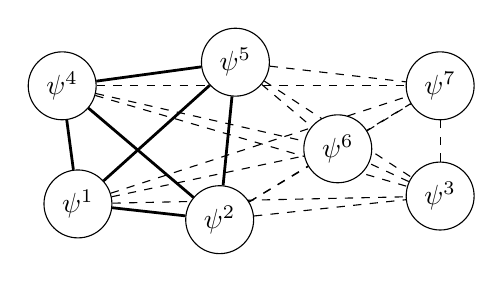
\begin{tikzpicture}[scale=1, transform shape]
	  \tikzstyle{every node} = [circle, draw, fill=white]
	  \node (1) at (0.2, 0.0) {$\psi^1$};
	  \node (2) at (2.0, -0.2) {$\psi^2$};
	  \node (5) at (4.8, 0.1) {$\psi^3$};
	  \node (4) at (0.0, 1.5) {$\psi^4$};
	  \node (3) at (2.2, 1.8) {$\psi^5$};
	  \node (6) at (3.5, 0.7) {$\psi^6$};
	  \node (7) at (4.8, 1.5) {$\psi^7$};
	  \begin{scope}[on background layer]
	  \foreach \from in {1,...,7}
	    \foreach \to in {\from,...,7}
	    \draw [dashed]  (\from) -- (\to);
	  \foreach \from in {1,...,4}
	    \foreach \to in {\from,...,4}
	    \draw [line width=1pt]  (\from) -- (\to);
	  \end{scope}
	\end{tikzpicture}
	\caption{\textbf{Illustration of the model.} Each node represents a fermion while each edge represents a connection through the Hamiltonian. Although edges imply pair-wise connections, each term in the Hamiltonian connects four at a time. For example, the $J_{1245}$ term is represented by the solid lines.}
	\label{fig:model}
\end{figure}

\subsection{$\cal{N}=1$ Supersymmetry}\emph{} \label{sub:N1susy}

The discussion of the supersymmetric models comes from reference~\cite{fu16}. In the $\cal N=1$ supersymmetric generalization, the Hamiltonian is written in terms of the single supercharge
\begin{align}
Q = i\sum_{i<j<k}C_{ijk}\psi^i\psi^j\psi^k,
\end{align}
where $C_{ijk}$ are now drawn from a Gaussian with mean 0 and variance $2J/N^2$. This is a $\hat{q} = 3$ model, where $\hat{q}$ is now the number of particles in each term of the supercharge. 

It might seem strange to define a supercharge when there are no bosonic operators. However, bilinear operators $\psi^i\psi^j$ behave like bosons because they do not change the fermion number. Operators 
\begin{align}
b^i = \acom{Q}{\psi^i} = \sum_{i<j<k}C_{ijk}\psi^j\psi^k, \quad \acom{Q}{b^i} 
	= 2Q\psi^iQ \label{eqn:N1bosons}.
\end{align}
can be interpreted as the bosonic operators.\footnote{I don't think this is right.}

The Hamiltonian is defined as
\begin{align}
H &= Q^2 = - \sum_{i<j<k}C_{ijk}\psi^i\psi^j\psi^k\sum_{\l<m<n}C_{\l mn}\psi^\l
	\psi^m\psi^n.
\end{align}
For those terms where $(i,j,k) = (\l,m,n)$, the sum becomes
\begin{align}
-\sum_{i<j<k} C_{ijk}^2 \psi^i\psi^j\psi^k \psi^i\psi^j\psi^k = \th{8} 
	\sum_{i<j<k}C_{ijk}^2.
\end{align}
For any term of the form $\psi^i\psi^j\psi^k\psi^i\psi^j\psi^\l = -\th{4}\psi^k\psi^\l$, there is one of the form $-\th{4}\psi^\l\psi^k=\th{4}\psi^l\psi^\l$ which cancels it. Therefore there are no quadratic terms in the Hamiltonian. Terms of the form $\psi^i\psi^j\psi^m\psi^k\psi^\l\psi^m = \th{2}\psi^i\psi^j\psi^k\psi^\l$ also match with their complements to form $\psi^k\psi^\l\psi^i\psi^j$, which in this case has the same sign as the former, leading to quartic terms
\begin{align}
-C_{ijm}C_{k\l m}\psi^i\psi^j\psi^k\psi^\l = -\th{8}C_{i[jm}C_{k\l]m} \psi^i \psi^j \psi^k\psi^\l,
\end{align}
with equality due to the antisymmetry of $C$ and the $\psi^i$. Lastly, any term with no matching $\psi$ also cancels with its complement, as in the quadratic case.

The Hamiltonian becomes
\begin{align}
H = E_0 + \sum_{i<j<k<\l}J_{ijk\l}\psi^i\psi^j\psi^k\psi^\l, \label{eqn:N1def}
\end{align}
where
\begin{align}
E_0 = \sum_{i<j<k} C_{ijk}^2\;,\qquad J_{ijk\l} = -\th{8}\sum_{a} C_{a[ij}
	C_{kl\l a}.
\end{align}
The $J_{ijk\l}$ terms connect the $N$ fermions, 4 at a time. Figure~\ref{fig:model} can also be used to represent this model.

This shows that $E_0$ is positive, with expectation (over the values of $C_{ijk}$)\footnote{There's still something not quite right here.}
\begin{align}
\ex{E_0} &= \sum_{i<j<k}\ex{C^2_{ijk}}\nn
&= \th{6}N(N-1)(N-2)\frac{2J}{N^2}.
\end{align}
In the large $N$ limit this becomes $E_0 = NJ/3$.\footnote{This contradicts the Fu paper's assertion that $E_0\to 0$ for large $N$. What am I missing?}

\subsection{$\cal{N}=2$ Supersymmetry}\emph{} \label{sub:N2susy}

In $\cal N=2$ supersymmetry, two supercharges are necessary. To create these, define a new set of fermions\footnote{Majorana or Dirac fermions?} that consists of $\psi^i$ and their conjugates $\bar{\psi_i}$. These obey the relations 
\begin{align}
\{\psi^i,\psi^j\} = 0, \quad \{\bar{\psi_i},\bar{\psi_j}\} = 0, \quad
	\{\psi^i,\bar{\psi_j}\} = \delta_j^i. \label{eqn:N2_ant}
\end{align}
The supercharges, with $\hat{q}=3$ still the number of fermions per term, are
\begin{align}
Q &= i\sum_{i<j<k}C_{ijk}\psi^i\psi^j\psi^k,\quad
\bar{Q} = i\sum_{i<j<k}\bar C^{ijk}\bar{\psi_i}\bar{\psi_j}\bar{\psi_k},
	\label{eqn:N2charge}
\end{align}
where the $C_{ijk}$ are complex numbers drawn from a 0-centered Gaussian such that
\begin{align}
\ex{C_{ijk}\bar C^{ijk}} = \frac{2J}{N^2}.
\end{align} 
The bosonic operators are defined as\footnote{Should this be antcommutation?}
\begin{align}
\bar{b}^i = \comm{Q}{\bar{\psi}_i}
\end{align}
An analysis similar to that in the previous subsection shows the Hamiltonian $H = \acom{Q}{\bar{Q}}$ can be written as
\begin{align}
H = E_0 + \sum_{ijk\l}J_{ij}^{k\l}\psi^i\psi^j\bar{\psi_k}\bar{\psi_\l}.
\end{align}
Like in the $\cal N=1$ case, the components of $J$ are no longer independent. 

The operators $Q^2$ and $\bar Q^2$ are both 0. That implies that both $Q$ and $\bar Q$ are conserved, as for example
\begin{align}
[H,Q] = Q\bar QQ + \bar QQQ - QQ\bar Q + Q\bar QQ = 0.
\end{align}
This also means they generate a symmetry of the Hamiltonian. This allows the methods of subsection~\ref{sub:susy} to be used to count ground states.

\section{$\cal{N}$ = 2 Ground States and Entropy} \label{sec:N2gs_ent}

The long-range order and large number of ground states in the $\cal N = 2$ supersymmetric model lead to nonzero entropy in subsystems of ground states, even at zero temperature. The high number of ground states and long-range correlation are intimately tied to this entropy.

\subsection{Counting Ground States} \emph{}\label{sub:count_gs}

A convenient way to bound the number of ground states from below is to partition the Hilbert space into energy eigenspaces with states connected by the supercharges, and show that any space with an odd number of states must be made of ground states. Consider a stationary state $\ket{\phi_E}$ with energy $E$. Consider also the states $\ket{q_E} = Q\ket{\phi_E}$ and $\ket{\bar q_E}= \bar Q \ket{\phi_E}$. These states will have the same energy eigenvalue $E$, if they exist. 

The two simple cases are if $\ket{q}$ and/or $\ket{\bar q}$ does not exist. If $Q$ and $\bar Q$ both annihilate $\ket{\phi_E}$, then $E=0$. If $\bar Q$ annihilates $\ket{\phi_E}$ but $Q$ does not, then 
\begin{align}
H\ket{\phi_E} = (Q\bar{Q} + \bar QQ)\ket{\phi_E} = \bar QQ\ket{\phi_E} = E\ket{\phi_E}
\end{align}
and the state $\ket{f_E} = \bar QQ\ket{\phi_E}$ is just $\ket{\phi_E}$, $E>0$. The same analysis applies if $Q$ annihilates but $\bar Q$ does not. These cases are illustrated in figure~\ref{fig:tuplets1}.

\begin{figure}
	\centering 
	\begin{tikzpicture}[scale=.9, transform shape]
	\tikzstyle{every node} = [rectangle]
	\node (phi)  at (1,0) {$\ket{\phi_E}$};
	\node (q)    at (0, 2) {$Q\ket{\phi_E}$};
	\node (qbar) at (2, 2) {$\bar Q\ket{\phi_E}$};
	\draw [->]   (phi) -- (q);
	\draw [->]   (phi) -- (qbar);
	\fill (3.5,.5) circle (1pt);
	\fill (3.5,1.5) circle (1pt);
	\node (phi)  at (6,0) {$\ket{\phi_a}$};
	\node (q)    at (5, 2) {0};
	\node (qbar) at (7, 2) {0};
	\draw [->]   (phi) -- (q);
	\draw [->]   (phi) -- (qbar);
	\node (,)    at (8.5,.5){,};
	\node (phi)  at (11,0) {$\ket{\phi_b}$};
	\node (q)    at (10, 2) {$\ket{q_b}$};
	\node (qbar) at (12, 2) {0};
	\node (E)    at (11, 4) {$\ket{f_{b}} = E_b\ket{\phi_b}$};
	\draw [->]   (phi) -- (q);
	\draw [->]   (phi) -- (qbar);
	\draw [->]   (q)-- (E);
	\end{tikzpicture}
	\caption{\textbf{Energy Eigenstate Tuplets} with either $Q$ or $\bar{Q}$ annihilating the states. Arrows up and to the left and right represent the effects of $Q$ and $\bar Q$, respectively. $\ket{\phi_a}$ must be a ground state. If $E_b\ne0$, then $\ket{f_{b}}=\ket{\phi_b}$ and the tuplet contains only two states.}
	\label{fig:tuplets1}
\end{figure}

If both $\ket{q_E}$ and $\ket{\bar q_E}$ exist and $E>0$, then
\begin{align}
H\ket{\phi_E} = E\ket{\phi_E} = (Q\bar Q + \bar QQ)\ket{\phi_E} = \ket{f_E} + 
	\ket{f'_E},
\end{align}
meaning 
\begin{align}
\ket{f_E} = \alpha\ket{\phi_E} + \beta\ket{\xi_E},\qquad \ket{f'_E} = 
	(1-\alpha)\ket{\phi_E} - \beta\ket{\xi_E}.
\end{align}
$\ket{q_E}$ and $\ket{\bar q_e}$ must be distinct, so $\ket{\xi_E}$ must exist. Therefore this tuplet also contains four states. Figure~\ref{fig:tuplets2} illustrates this case.

\begin{figure}
	\centering 
	\begin{tikzpicture}[scale=.9, transform shape]
	\tikzstyle{every node} = [rectangle]
	\node (phi)  at (1,0) {$\ket{\phi_E}$};
	\node (q)    at (0, 2) {$Q\ket{\phi_E}$};
	\node (qbar) at (2, 2) {$\bar Q\ket{\phi_E}$};
	\draw [->]   (phi) -- (q);
	\draw [->]   (phi) -- (qbar);
	\fill (3.5,.5) circle (1pt);
	\fill (3.5,1.5) circle (1pt);
	\node (phi)  at (7, 0) {$\ket{\phi_c}$};
	\node (q)    at (5, 2) {$\ket{q_c}$};
	\node (qbar) at (9, 2) {$\ket{\bar{q}_c}$};
	\node (f)    at (6, 4) {$\ket{f_c}$};
	\node (fpr)  at (8, 4) {$\ket{f_c'}$};
	\draw [->]   (phi)  -- (q);
	\draw [->]   (phi)  -- (qbar);
	\draw [->]   (q)    -- (f);
	\draw [->]   (qbar) -- (fpr);
	\end{tikzpicture}
	\caption{\textbf{Energy Eigenstate Tuplets} with neither $Q$ nor $\bar{Q}$ annihilating the states. Since $\ket{f_c}$ and $\ket{f_c'}$ must be distinct (otherwise $\acom{Q}{\bar{Q}}\ket{\phi_c}=Q^2\ket{\phi_c} = 0$), they each must be linear combinations of $\ket{\phi_c}$ with another state $\ket{\xi_c}$.}
	\label{fig:tuplets2}
\end{figure}

The previous analysis divides the space into tuplets of energy eigenstates with at most 4 members. All tuplets contain an even number of states, except for the ground state tuplets. All even tuplets contain an equal number of fermionic and bosonic states because the supercharges interchange bosonic states with fermionic states. This shows that the supersymmetry is unbroken, as described in subsection~\ref{sub:susy}.

This provides the opportunity to count ground states using the Fermi number
\begin{align}
F = \sum_i\bar{\psi_i}\psi^i,
\end{align}
which is even for bosonic states and odd for fermionic states. For all paired subspaces with non-zero energy, the Witten index 
\begin{align}
W = \Tr\left((-1)^F\right) 
	\label{eqn:N2witten}
\end{align}
evaluates to 0. Then the trace over the whole space has contributions only from the ground states, so the number of ground states will be equal to or greater than $|W|$. As a result, the modified Witten index $\Tr\left((-1)^F\e^{\beta H}\right)$ is independent of temperature $1/\beta$ because $H$ is zero in the ground states. 

Define the unitary operator 
\begin{align}
R^p = \e^{\frac{2\pi ipF}{\hat q}},\quad R^3 = \mathbb{1}.
\end{align}
$R$ commutes with $Q$ so that $\Tr\left((-1)^FR^p\right)$ also only has contributions from the ground state. This defines a modified Witten index
\begin{align}
W_p = \Tr\left((-1)^FR^\frac{2\pi ip}{\hat q}\right).
\end{align}
Since $W$ is independent of the coupling, the Hamiltonian can be turned off, in which case the index is just the product of the indexes over all particles $\left(Z^{(1)}\right)^N$ so that 
\begin{align}
W_p = \left(1-\e^{\frac{2\pi ip}{3}}\right)^N = e^{i\pi N\left(\frac{p}{\hat q} - \th{2}\right)}\left(2\sin\frac{\pi p}{\hat q}\right)^N
\end{align}
and the degeneracy of the ground state is 
\begin{align}
D_\text{GS} \ge \abs{W} = \left(2\sin\frac{\pi p}{\hat q}\right)^N. \label{eqn:dgs}
\end{align}
To provide the highest bound on $D_\text{GS}$, choose $p = (\hat q+1)/2$, so that $D_\text{GS} \ge \sqrt{3}^N$, where $\hat q = 3$ for the supercharge in equation~\ref{eqn:N2charge}.

Compare this to the total number of states $2^N$. It is clear that the number of ground states is extensive, as the number of degrees of freedom, the log of $D_\text{GS}$, scales linearly with $N$.

\subsection{Ground State Entanglement Entropy} \emph{} \label{sub:entangle}

The large number of ground states has an interesting effect on the entanglement entropy of a subsystem of a ground state. Classically, entropy measures uncertainty about an event or state. The nearest quantum mechanical analogue is Von Neumann entropy
\begin{align}
S = -\Tr(\rho\log\rho).\label{eqn:vnent}
\end{align}
Written in the eigenbasis of $\rho$, this becomes 
\begin{align}
S = -\sum_ip_i\log p_i,\quad \rho = \sum_i p_i\ket{i}\bra{i},
\end{align}
which mimics the classical form.

The entropy of a pure state is always 0. However, subsystems of a pure state are mixed, and therefore have non-zero entropy. This entropy does not represent uncertainty, since the state of the whole system is known. Rather, it represents the classical information one system can gain about the other through a local measurement~\cite{janzing09}.

\begin{figure}
	\centering
	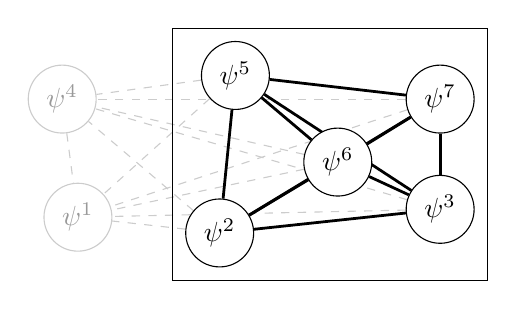
\begin{tikzpicture}
	  \tikzstyle{every node} = [circle, draw=black!20, fill=white]
	  \node (7) at (0.2, 0.0) {\textcolor{mygray}{$\psi^1$}};
	  \node (5)[draw=black] at (2.0, -0.2) {{$\psi^2$}};
  	  \node (1)[draw=black] at (4.8, 0.1) {$\psi^3$};
  	  \node (6) at (0.0, 1.5) {\textcolor{mygray}{$\psi^4$}};
	  \node (4)[draw=black] at (2.2, 1.8) {{$\psi^5$}};
	  \node (2)[draw=black] at (3.5, 0.7) {$\psi^6$};
	  \node (3)[draw=black] at (4.8, 1.5) {$\psi^7$};
	  \begin{scope}[on background layer]
	  \foreach \from in {1,...,7}
	    \foreach \to in {\from,...,7}
	    \draw [dashed, color=black!20]  (\from) -- (\to);
	  \foreach \from in {1,...,5}
	    \foreach \to in {\from,...,5}
	    \draw [line width=1pt]  (\from) -- (\to);
	  \end{scope}
	  \draw (1.4, -.8) rectangle (5.4, 2.4);
	\end{tikzpicture}
	\caption{\textbf{Subsystem of the Model.} If fermions 1 and 4 are traced out, the resulting density matrix describes the relationships between the others.}
	\label{fig:subsys}
\end{figure}

Consider state $\ket{\phi}_\cal{A}$ on a system $\cal A$ that can be decomposed into subsystems $A$ an $B$. The state can in general be written as 
\begin{align}
\ket{\phi}_\cal{A} = \sum_jc_j\ket{\phi_j}_A\ket{\phi_j}_B,
\end{align}
where the $\ket{\phi_j}$ are orthogonal in each subsystem. Then $j$ can only run over the dimension $m$ of the smaller subspace. Since the reduced density matrices $\rho_A = \Tr_B\rho_{\cal A}$ are
\begin{align}
\rho_A = \sum_jp_j\ket{\phi_j}_A\bra{\phi_j}_A, \quad \rho_B = \sum_jp_j\ket{\phi_j}_B\bra{\phi_j}_B; \quad p_j = |c_j|^2,
\end{align}
It is clear that the entropies of entanglement are equal for each subsystem. In fact, they satisfy 
\begin{align}
S(\rho) = S(\rho_B) = \cal{H}(p_j),
\end{align}
where $\cal H$ is the classical Shannon entropy with $p_j$ interpreted as classical probabilities. 

A general ground state in the $\cal N=2$ SYK model can be written as 
\begin{align}
\ket{\phi_0} = \sum_ic_i\ket{i}_A\ket{i}_B. \label{eqn:mixed}
\end{align}
If the smaller of the two subsystems has $m$ particles, the sum in~\ref{eqn:mixed} can contain at most $2^m$ terms, the maximum number of states in the smaller subsystem. Maximum entropy is achieved when the coefficients are equal, so 
\begin{align}
S_\text{max} = \sum_{i=1}^{2^m}\th{2^m}\log 2^m = m\log(2).\label{eqn:thermal}
\end{align}
This is a general bound on the bipartite entanglement entropy of any system.

At $T=0$, the entropy should be $S = \log D_\text{GS} = N\log\sqrt{3} $~\cite{fu16}.\footnote{Is this the bipartite entanglement entropy or something else?}

\section{Numerical Results} \label{sec:numeric}

Computations on the $\cal N=2$ model were completed in Python using Numpy~\cite{vander11}.

\subsection{Building Matrices}\emph{} \label{sub:build_mat}

The simplest way to compute large-N functions on a computer is to use a matrix representation for the group. This can be done by viewing the $\bar \psi$ and $\psi$ operators as raising and lowering operators, respectively. Consider the case of $N$ fermions. Write the state as an $N$-dimensional binary vector
\begin{align}
\ket{m} = \ket{m_1m_2\dots m_i\dots m_{N-1}m_N}, \quad\sum_im_i2^{i-1} =
	m.\label{eqn:2Nstate}
\end{align}
The vacuum state is $\ket{0}$. A populated state can be written as
\begin{align}
\ket{110\dots 0} = \bar\psi_1\bar{\psi_2}\ket{0} =-\bar\psi_2\bar\psi_1\ket{0},
\end{align}
which enforces the canonical ordering through anticommutation relations. 

The matrix representations of $\psi^i, \bar \psi_i$ are then calculated component-wise as a $2^N$ by $2^N$ matrix.
\begin{align}
\bar\psi_i &= \sum_{a,b}\ket{a}\bar\psi_{i,ab}\bra{b}\nn
\bar\psi_{i,ab} &= \brakett{a}{\bar\psi_i}{b}.\label{eqn:comps}
\end{align}
These components may be calculated effectively using the pseudocode in figure~\ref{code:psibar}.

\begin{figure}[ht]
	\begin{lstlisting}[language=python][gobble=2]
    def psi_bar(N,i):
      psi_bar = np.zeros((2^N,2^N))
      for (n,m) in psi_bar:
        if (m-n == 2^j) and (n & 2^j == 0): 
          psi[m,n] = (-1)^Fermi(n,j),
    return psi_bar
	\end{lstlisting}
	\cprotect\caption{\textbf{Code for generating $\bar \psi$ matrices,} where \verb|^| represents exponentiation, \verb|&| represents bitwise and \verb|Fermi(n,j)|, the reduced Fermi number, is the number of nonzero components in \verb|n| before the \verb|j|'th component. This handles anticommutation requirements. A similar structure can be used for building the $\psi$ matrices.}
	\label{code:psibar}
\end{figure}

It is also possible to create the matrices recursively. The base case is $N=1$, for which the matrices are the raising and lowering matrices,
\begin{align}
\bar\psi_{1,(1)} = \begin{bmatrix} 0&0\\1&0 \end{bmatrix}, \qquad
    \psi^1_{(1)} = \begin{bmatrix} 0&1\\0&0 \end{bmatrix}. \label{eqn:base}
\end{align}
Then, to increase the dimension take the tensor product with the $2\times 2$ identity matrix $I$,
\begin{align}
\bar\psi_{i,(N)} = I\otimes\bar\psi_{i,(N-1)},\quad \psi^i_{(N)} = I\otimes 
	\psi^i_{(N-1)}.
\end{align}
This formula of course does not work when $i=N$. In this case the solution is still to use recursion, with the formula
\begin{align}
\bar\psi_{i,(N)} = \bar\psi_{i-1,(N-1)}\otimes\sigma_3,
\end{align}
with equation~\ref{eqn:base} again supplying the base case.

Although there are various representations of the group, the previous two constructions lead to the same representation. The analysis in this paper used the former method because of its relative simplicity.

\subsection{Ground States} \emph{} \label{sub:num_gs}

Counting ground states was implemented by counting the zero eigenvalues of a randomly-generated Hamiltonian. The number of ground states stayed above the bound in equation~\ref{eqn:dgs}, although the bound was not tight in some places. See figure~\ref{fig:gserr} for the number of ground states above the bound.

\begin{figure}
	\centering
	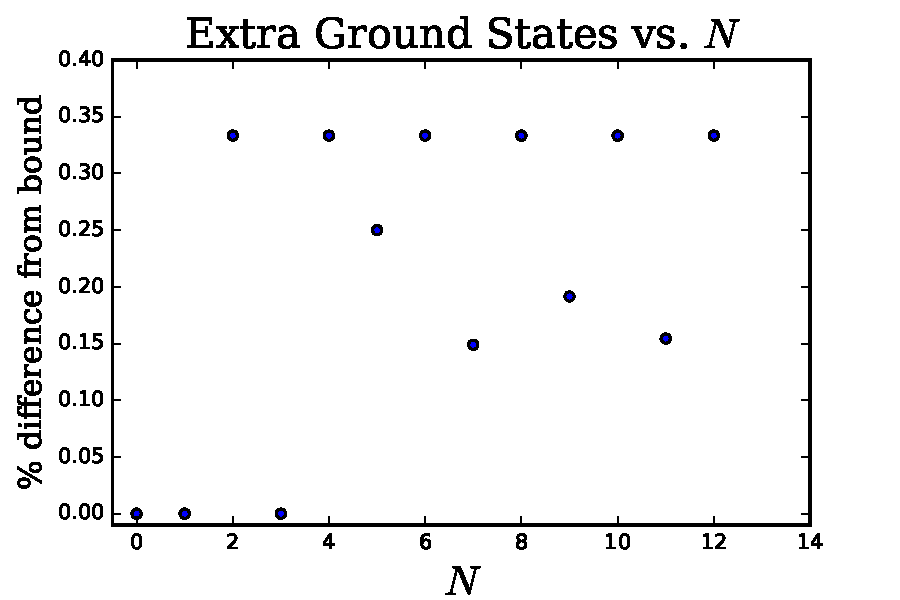
\includegraphics[width=.5\textwidth]{gserr}
	\caption{\textbf{Looseness of bound on number of ground states.} 0 represents the bound being tight while 1 would mean twice as many ground states as the bound. Since the number of ground states is an integer, these values were calculated as $\text{ceil}(\sqrt{3}^N)$.}
	\label{fig:gserr}
\end{figure}

It is particularly interesting to note that the number of ground states is particularly high for even $N$. Even with randomly generated Hamiltonians, the relative number of ground states above the bound stays relatively constant near 0.33 in this case.

\subsection{Ground State Entanglement Entropy}\emph{} \label{sub:num_ent}

Once the number of ground states were calculated for a single Hamiltonian, the entropy of a subsystem of the ground state could be calculated from the reduced density matrix of the subsystem. Starting with a ground state $\ket{\phi}$, the density matrix $\rho = \ket{\phi}\bra{\phi}$ can be calculated. The entropy $S = \Tr\rho\log\rho$ can be calculated as 
\begin{align}
S = \sum \lambda\log\lambda,
\end{align}
where $\lambda$ are the eigenvalues. 

As predicted, the entropy rises and drops linearly as more particles are traces over. Since the ground states depend on the coupling, it is necessary to perform multiple calculations and average the entropies. 

To see the symmetric linear dependence of the entropy on size of subspace, see figure~\ref{fig:N11pred_ent}. The solid line shows the entropy of a thermal state as defined in equation~\ref{eqn:thermal}. Figure~\ref{fig:allentropy} shows entropy of the reduced density matrices for $N = 1,2,3...11$. When one partition is smaller than the other, the $m\log2$ bound is close to tight. 

\begin{figure}
	\centering
	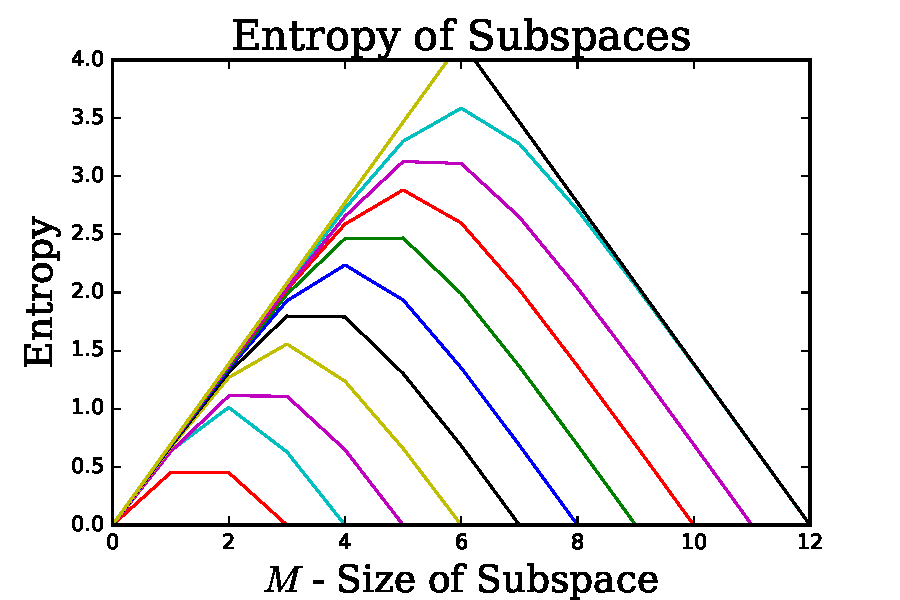
\includegraphics[width=.5\textwidth]{allentropy}
	\caption{\textbf{Entanglement Entropy.} Each curve shows the entropy for a given $N$ at various $M$. The straight line bounds the entropy as $m\log2$.}
	\label{fig:allentropy}
\end{figure}

Close to equipartition, the entropy is smaller. Figure~\ref{fig:maxentropy} shows the maximum entropy as a function of $N$.

\begin{figure}
	\centering
	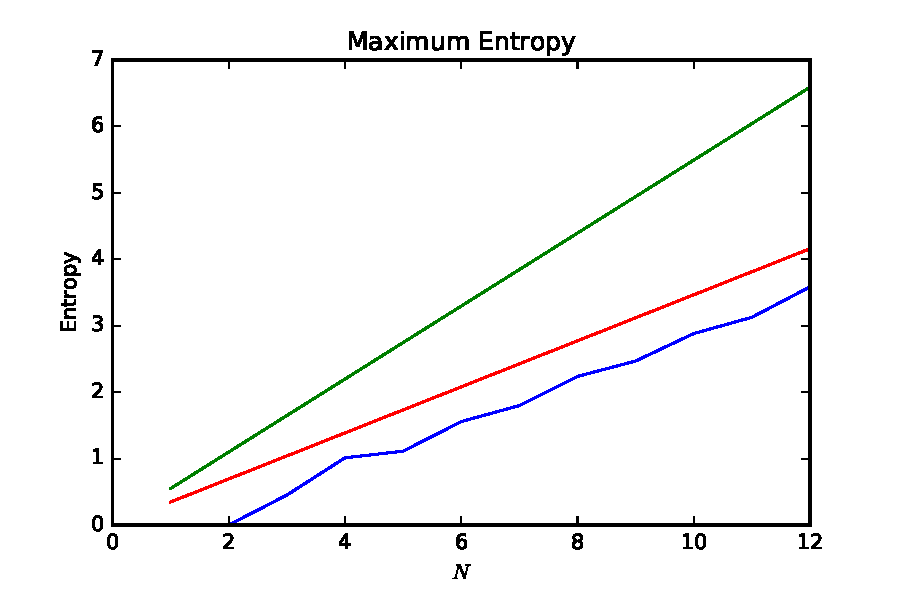
\includegraphics[width=.5\textwidth]{maxentropy}
	\caption{\textbf{Maximum Entropy.} }
	\label{fig:maxentropy}
\end{figure}

\section{Conclusion} \label{sec:concl}

Interesting future work for this project could include running similar calculations for the $\cal N=1$ model and running calculations for higher $N$. The $\cal N=1$ calculations would not be very different to set up, but would have different results because of the difference in the theories, especially due to the broken supersymmetry at small $N$. Calculations for larger $N$ could be made efficient by exploring alternative ways to create the $\psi$ matrices, or writing code in a different language.

Another aspect to explore is the holographic dual of these results.

\printbibliography

\end{document}
